
In the following, we will summarise the results obtained for the IRTF
data set. We deal with the different physical paramenters in separate
Sections. We start by reporting the Root Mean/Median Square Errors
(RMSE/RMDSE) with respect to the parameters gathered from the
literature by \cite{cesetti} and included in their Table 3.

\subsection{Effective temperature models}

Table \ref{tab:model_TSD} summarises the RMSE/RMDSE for the complete
set of models: the minimum $\chi^2$ estimate based on the full
spectrum ($\chi^2$), the projection pursuit regression based on the
ICA components (PPR-ICA) and models trained on the spectral features
proposed by the GA (GA-RF, GA-GBM, GA-SVR, GA-NNET, GA-MARS,
GA-KPLS, GA-RR). For each model, we report the RMSE/RMDSE obtained for
several noise levels of the training sets.  SNR=$\infty$ corresponds
to noiseless spectra. In the GA- cases, the model is trained with
  the spectral features found by the Genetic Algorithms when applied
  to BT-Settl spectra of the corresponding SNR.

{\bf Make sure we always have Rule-Regression models everywhere or
  discuss why not.}
  
\newcommand{\ra}[1]{\renewcommand{\arraystretch}{#1}}
\begin{table*}\centering
\ra{1.3}
\begin{tabular}{@{}lrrcrrcrr@{}}\toprule
& \multicolumn{2}{c}{$SNR = 10$} & \phantom{ab}& \multicolumn{2}{c}{$SNR = 50$} &
\phantom{ab} & \multicolumn{2}{c}{$SNR = \infty$}\\
\cmidrule{2-3} \cmidrule{5-6} \cmidrule{8-9}
$Regression Models$ & $RMSE$ & $RMDSE$ && $RMSE$ & $RMDSE$ && $RMSE$ & $RMDSE$ \\ \midrule
$\chi^2$      & 232      & \bf{100}&& 235      & 120    && 232      & \bf{100} \\
 PPR-ICA      & 242      & 128        && 242      &  99    && 280      & 162 \\
 GA-RF        & 308      & 183        && 248      & 136    && \bf{167} & 135 \\
 GA-GBM       & 287      & 160        && 248      & 149    && 233      & 113 \\
 GA-SVR       & \bf{221} & 122        && 281      & 151    && 299      & 160 \\
 GA-NNET      & 283      & 192        && 264      & 114    && 326      & 212 \\
 GA-KNN       & 238      & 120        && \bf{232} & 137    && 219      & \bf{100}  \\
 GA-MARS      & 253      & 113        && 254      & \bf{95}&& 226      & 133 \\
 GA-KPLS      & 275      & 120        && 300      & 119    && 387      & 218 \\
\bottomrule
\end{tabular}
\caption {Cross-validation RMSE and RMDSE for the various regression
  models that predict $T_{eff}$ (K).}
\label{tab:model_TSD} 
% \end{center}
\end{table*}

Table \ref{tab:model_TSD} shows that the performance of classifiers
based on the full spectrum (or in a compressed version in the form of
ICA components) and the best classifier based on features derived from
limited spectral bands is equivalent. The bartlett test shows that the
variances are homogeneous with a Bartlett\textquoteright s K-squared
of 8.5 with 2 degrees of freedom and a p-value of0.01426. The
Flinger-Killen test shows that homokedascity is verified at the
p=0.005886 level. Finally, the F-ANOVA test clearly shows that there
is no significant difference between models. Thus, we conclude that
the quality of features from the two approaches are equivalent in
predictive performance.  The difference between the performances of
the best classifier ($GA-KNN$; best on average over SNR), the minimum
$\chi^2$ classifier, and the $PPR-ICA$ classifiers are not
statistically significant. The bartlett test shows that the variances
are homogeneous with a Bartlett\textquoteright s K-squared of 8.5 with
2 degrees of freedom and a p-value of0.01426. The Flinger-Killen test
shows that homokedascity is verified at the p=0.005886 level. Finally,
the F-ANOVA test clearly shows that there is no significant difference
between models. Thus, we conclude that the quality of features from
the two approaches are equivalent in predictive performance.  In any
case, it is evident that the RMSE is significantly above the grid
spacing in temperature. We interpret the small differences as an
indication that there is as much information spread over the entire
spectrum shape as can be distilled from a few spectral bands.

The comparison with the effective temperatures compiled by
\cite{cesetti} shows however some significant differences across
models when evaluated not by the RMSE/RMDSE, but by the average bias
(see Table \ref{tab:model_Tbias}). 

\begin{table*}\centering
\ra{1.3}
\begin{tabular}{@{}lrrr@{}}\toprule
& {$SNR = 10$} & {$SNR = 50$} & {$SNR = \infty$}\\ \midrule
$\chi^2 $            &  -77 &  -87  & -85 \\
$ICA+ppr$            & -104 & -55   & -130 \\
GA-RR                & -102 &  -39  & 170 \\
GA-RF                & -173 & -127  &  -5 \\
GA-GBM               & -141 & -109  &  32 \\
GA-SVR               &  -58  &  -3  &  92 \\
GA-NNET              & -147 &  -36  &  39 \\
GA-KNN               &  -76  &-110  & -67 \\
GA-MARS              &  -57  & -88  &  98 \\
GA-KPLS              & -120 &   -4  & 214 \\
\bottomrule
\end{tabular}
\caption {Average bias in the $T_{eff}$ (K) estimates computed with
  respect to the reference values in Table 3 of \cite{cesetti}.}
\label{tab:model_Tbias} 
% \end{center}
\end{table*}

In general, all classifiers tend to predict lower effective
temperatures than those in the literature except in the noiseless
scenario. The models trained with noiseless spectra tend to
overestimate $T_{\rm eff}$, suggesting that the optimal SNR is between
SNR=50 and $\infty$. The minimum-$\chi^2$ approach and the GA-KNN
model systematically underestimate $T_{\rm eff}$ for all SNR
regimes. This shared behaviour is not surprising since minimum
$\chi^2$ is a single nearest neighbour method applied in the space of
the entire spectrum as opposed to the space selected features.

We have found in previous studies that, at least for input spaces
constructed from ICA compressions of the spectra, it is not necessary
to adapt the training set SNR to match exactly that of the prediction
set. On the contrary, we find that two regimes are sufficient to
obtain acceptable results. The two regimes are separated at
SNR=10. The model trained with SNR=50 spectra gives close to optimal
results for spectra with SNRs above 10, while below that limit the
same situation holds for the model trained with SNR=10 spectra. {\bf
  Cite paper by Ana.}

In Figures~\ref{fig:comp01}~\ref{fig:comp02} the relationship between
Temperature estimated from the GA technique proposed features and
modeled with different techniques and the $chi^2$ with SNR=50 against
the estimations provided by \cite{cesetti} can be seen.

\begin {figure}
 \centering
 \begin{subfigure}{.85\textwidth}
  \centering
  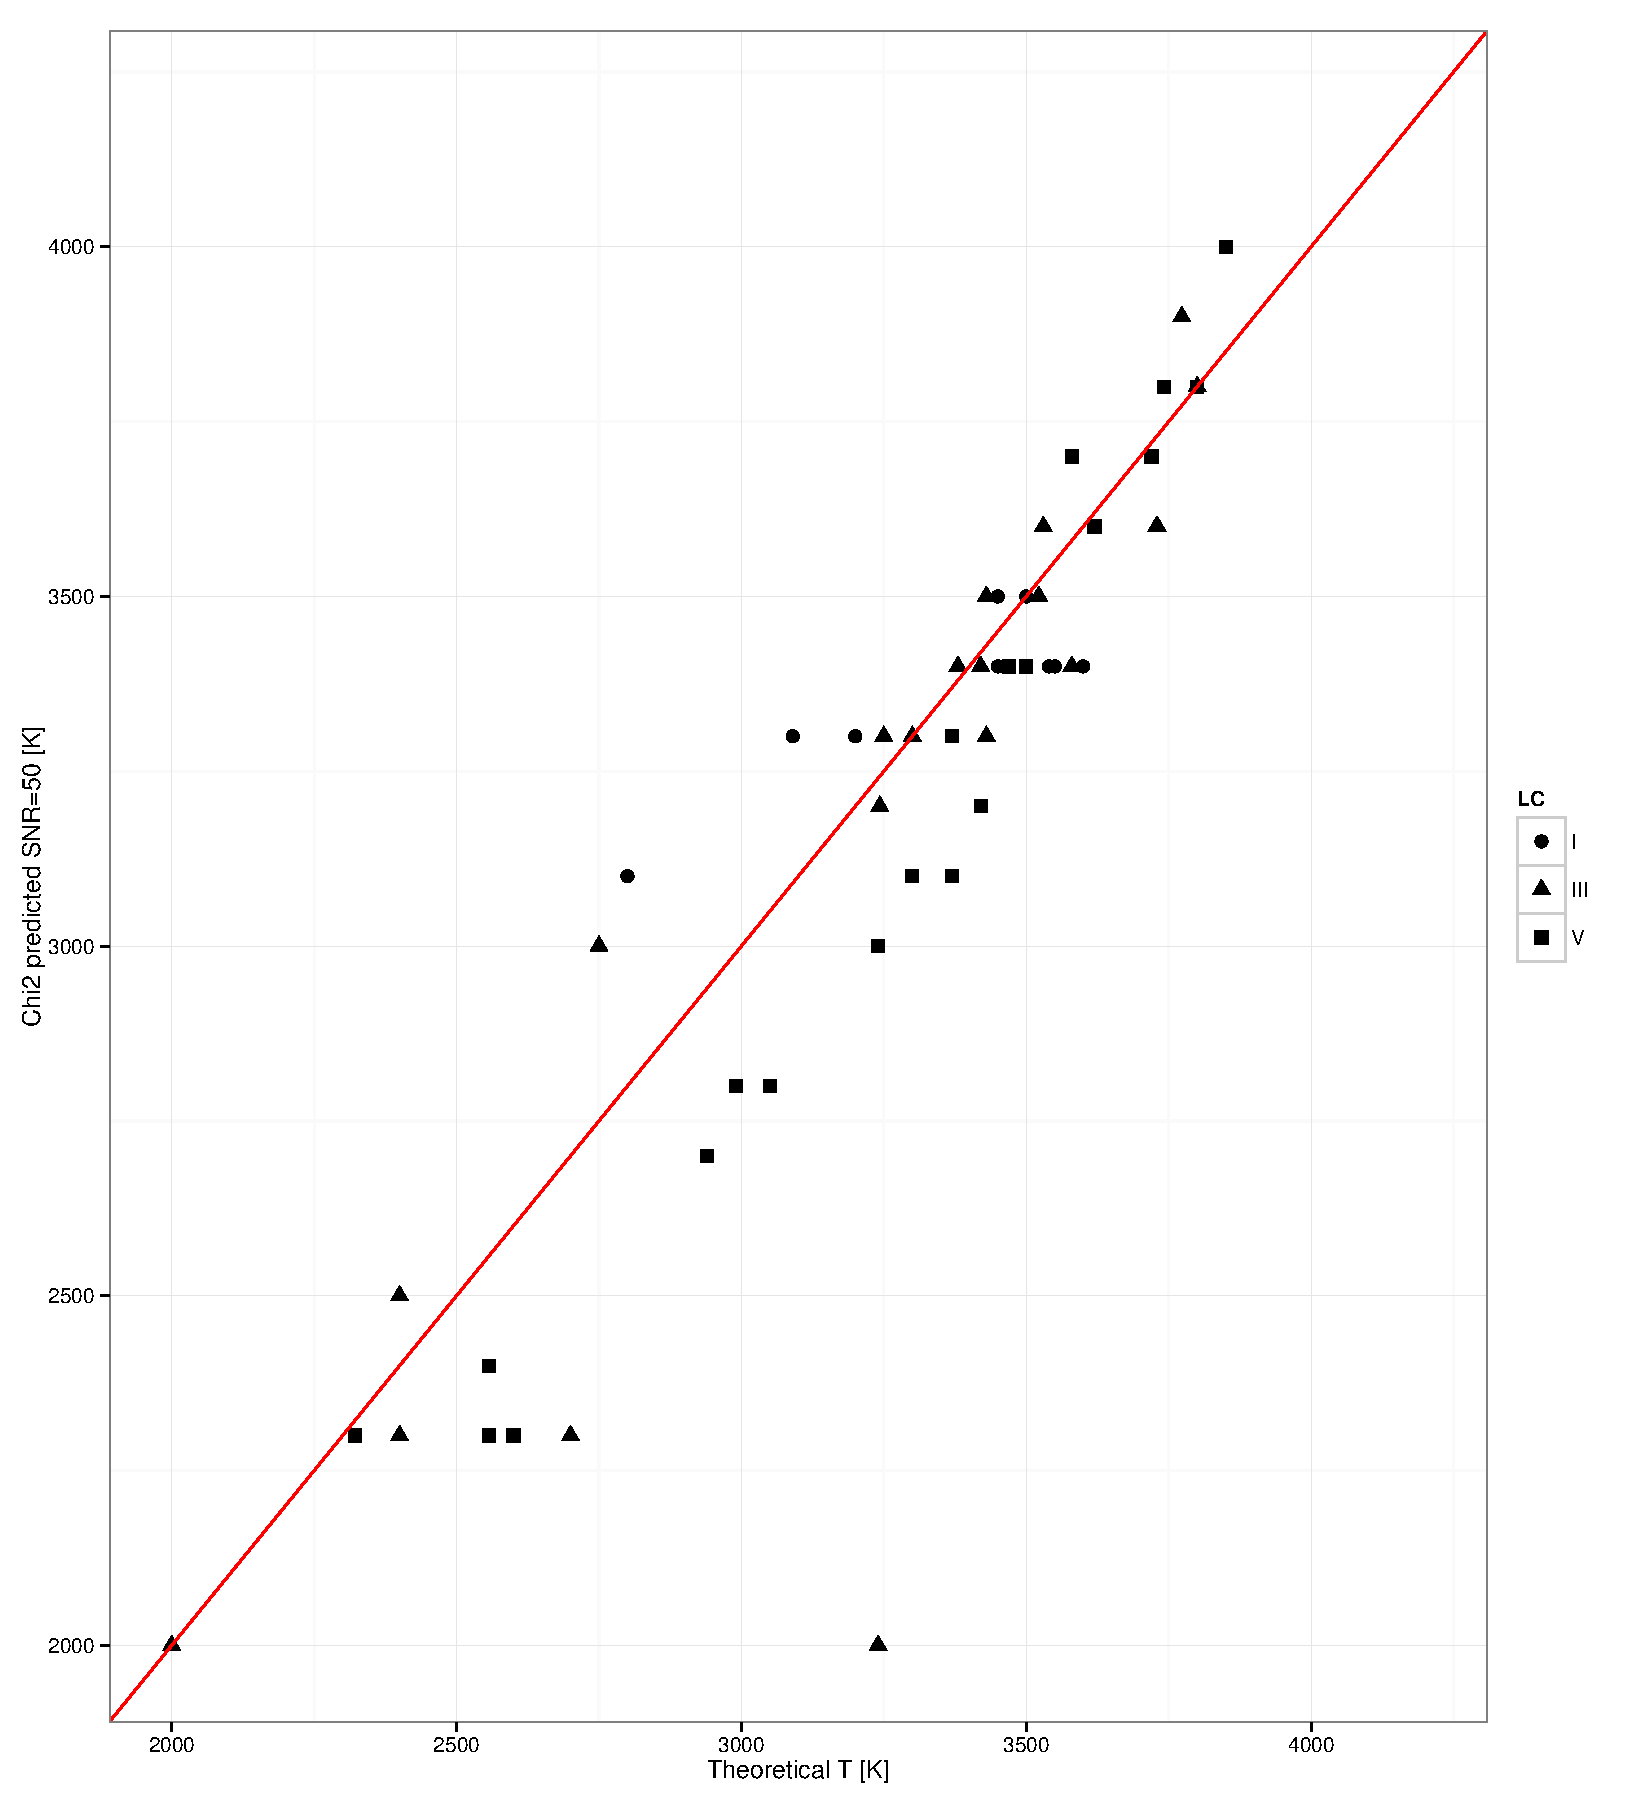
\includegraphics[width=11cm]{figs/irtf_T_chi250_Cesetti.pdf}
  \caption{Comparison between Temperature estimations from Cesetti 
  in x axis and the closest BT\_Settl spectra by $\chi^2$ at SNR=$50$ on y-axis}
 \label{fig:chi2_50_spt}
 \end{subfigure}
  \begin{subfigure}{.85\textwidth}
  \centering
  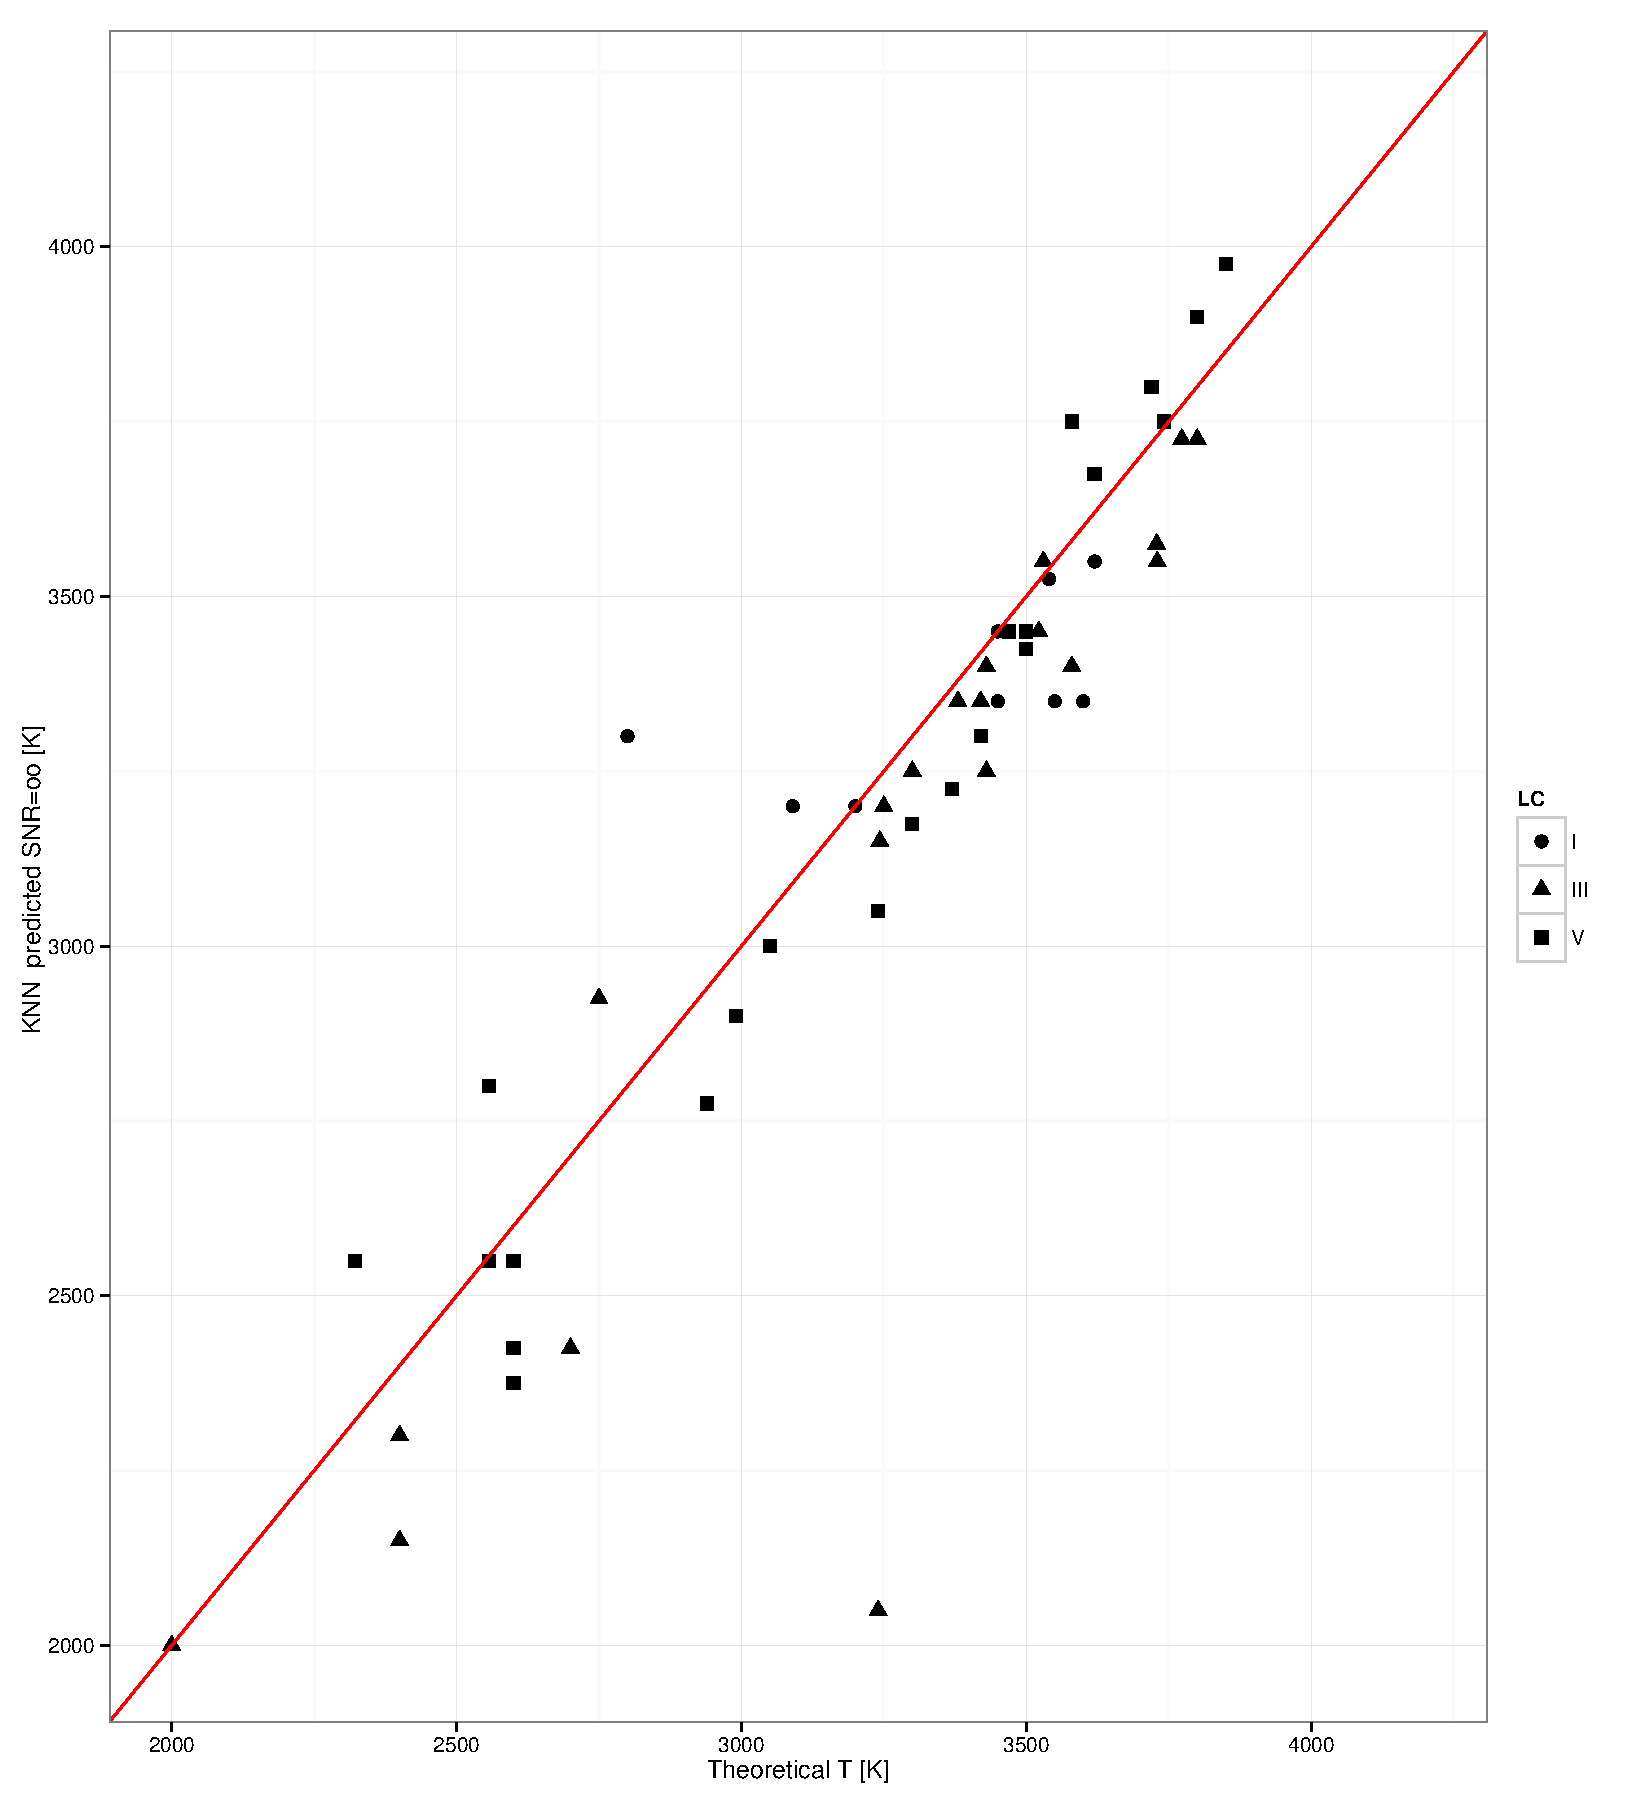
\includegraphics[width=11cm]{figs/irtf_T_knnoo_Cesetti.pdf}
  \caption{Comparison between Temperature estimations from Cesetti 
 in x axis and the KNN model for GA based features 
 at SNR=$\infty$ on y-axis}
 \label{fig:ga_too50ga_spt}
 \end{subfigure}
 \label {fig:comp01}
 \caption{Performance comparison between the $\chi^2$ based selection 
          and the band oriented features}
\end {figure}
 
 
\begin {figure}
 \centering 
 \begin{subfigure}{.85\textwidth}
  \centering
  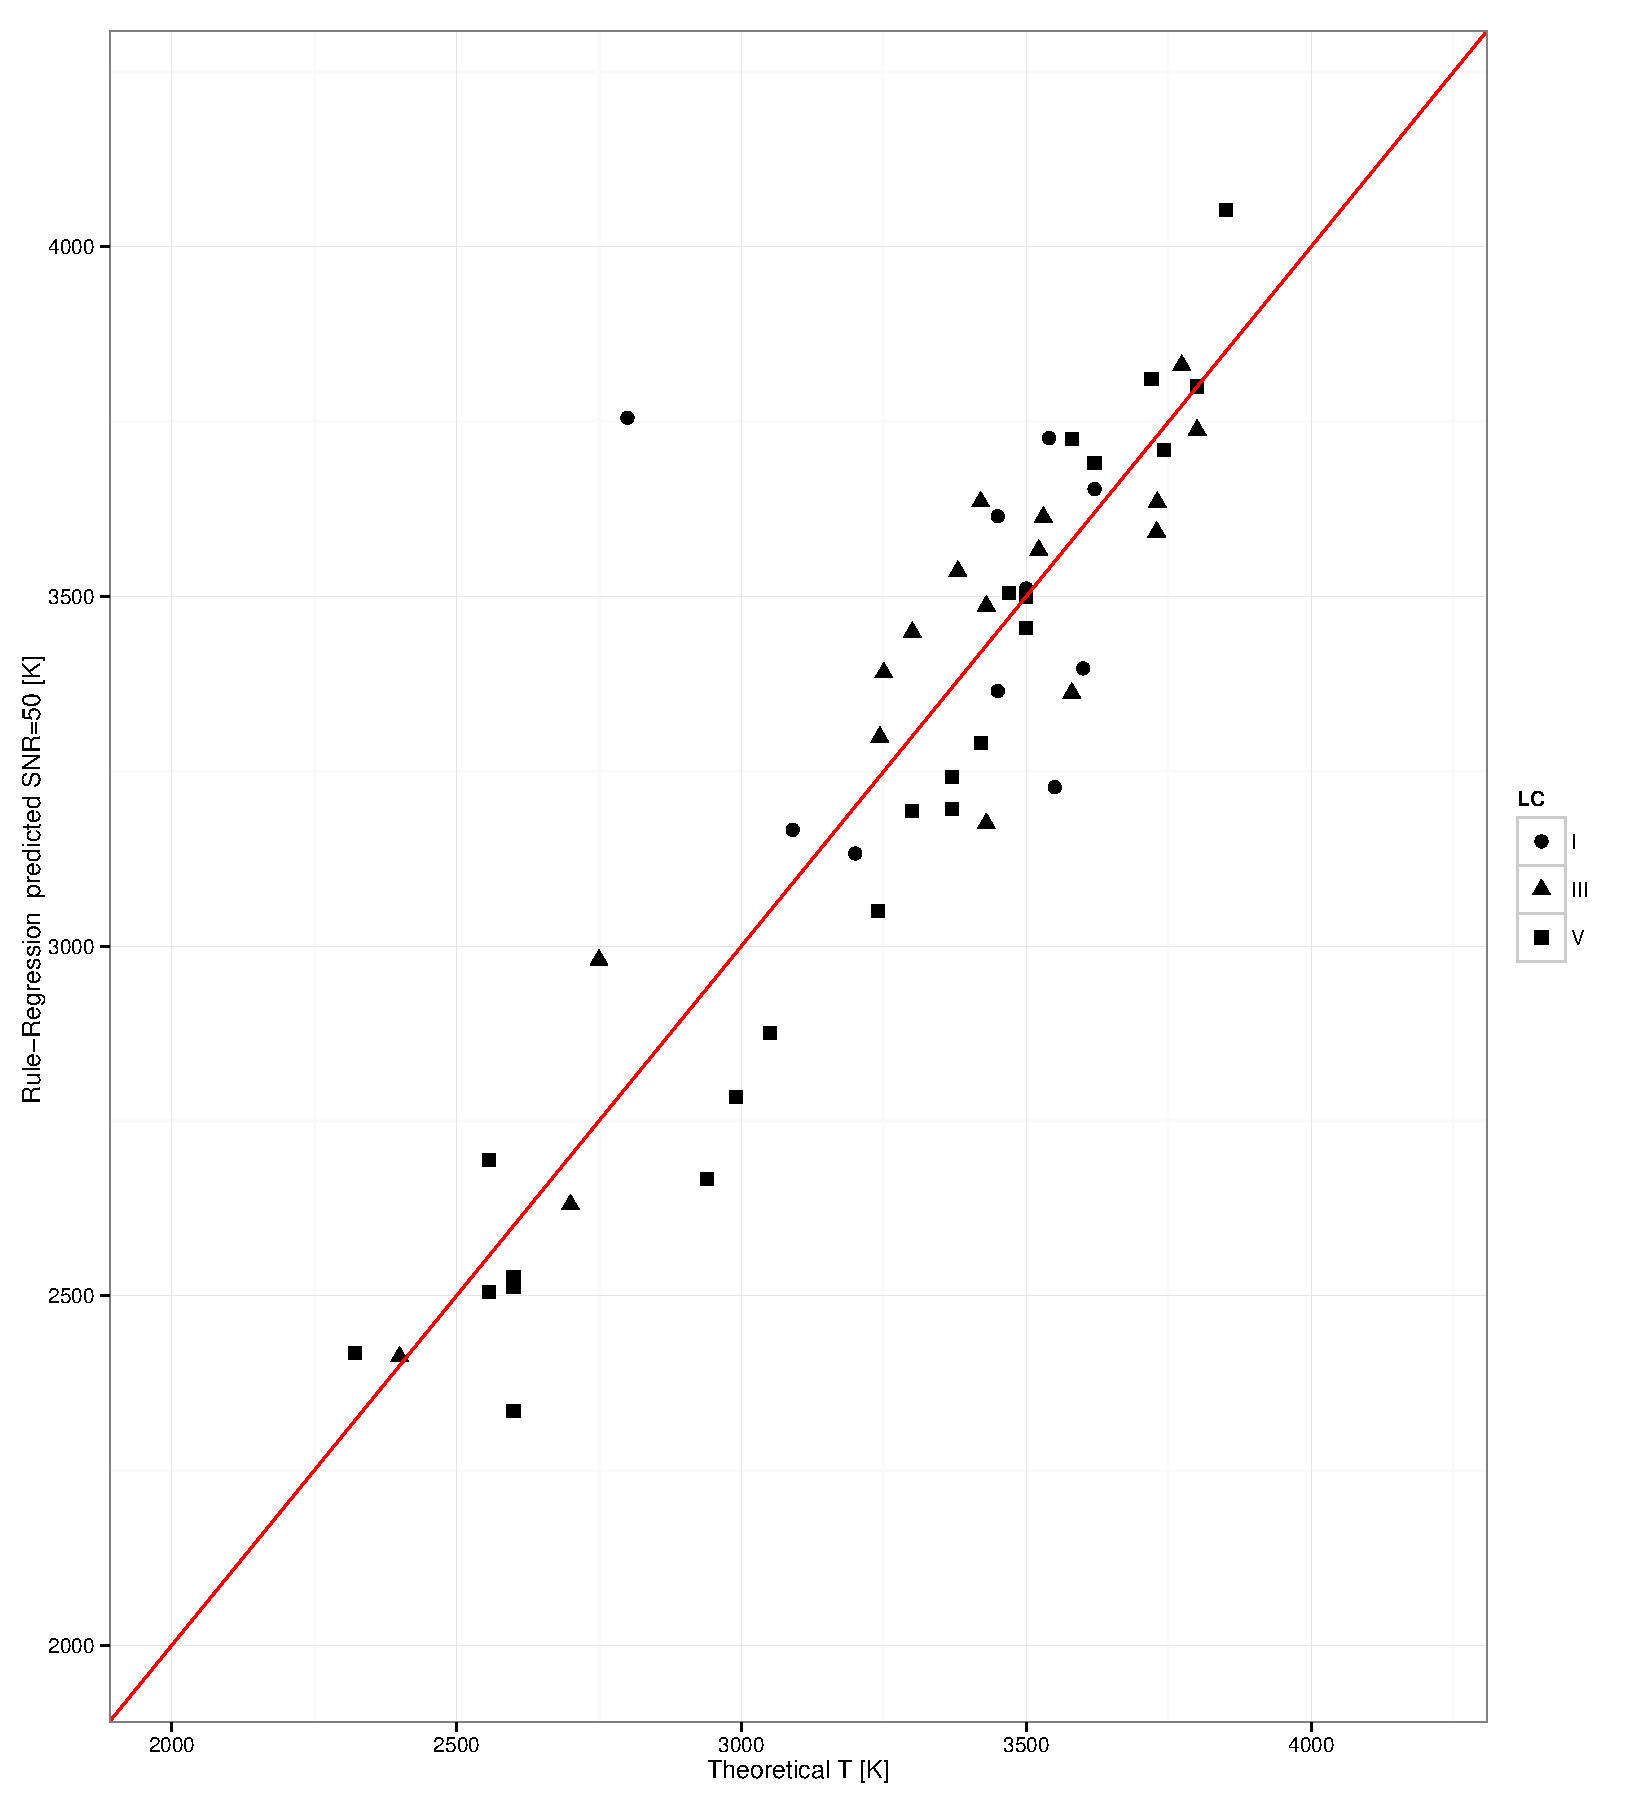
\includegraphics[width=11cm]{figs/irtf_T_rregoo_Cesetti.pdf}
  \caption{Comparison between Temperature estimations from Cesetti 
 in x axis and the Rule Regression model for GA based features 
 at SNR=$\infty$ on y-axis}
 \label{fig:ga_rr00ga_spt}
 \end{subfigure}
\begin{subfigure}{.85\textwidth}
  \centering
  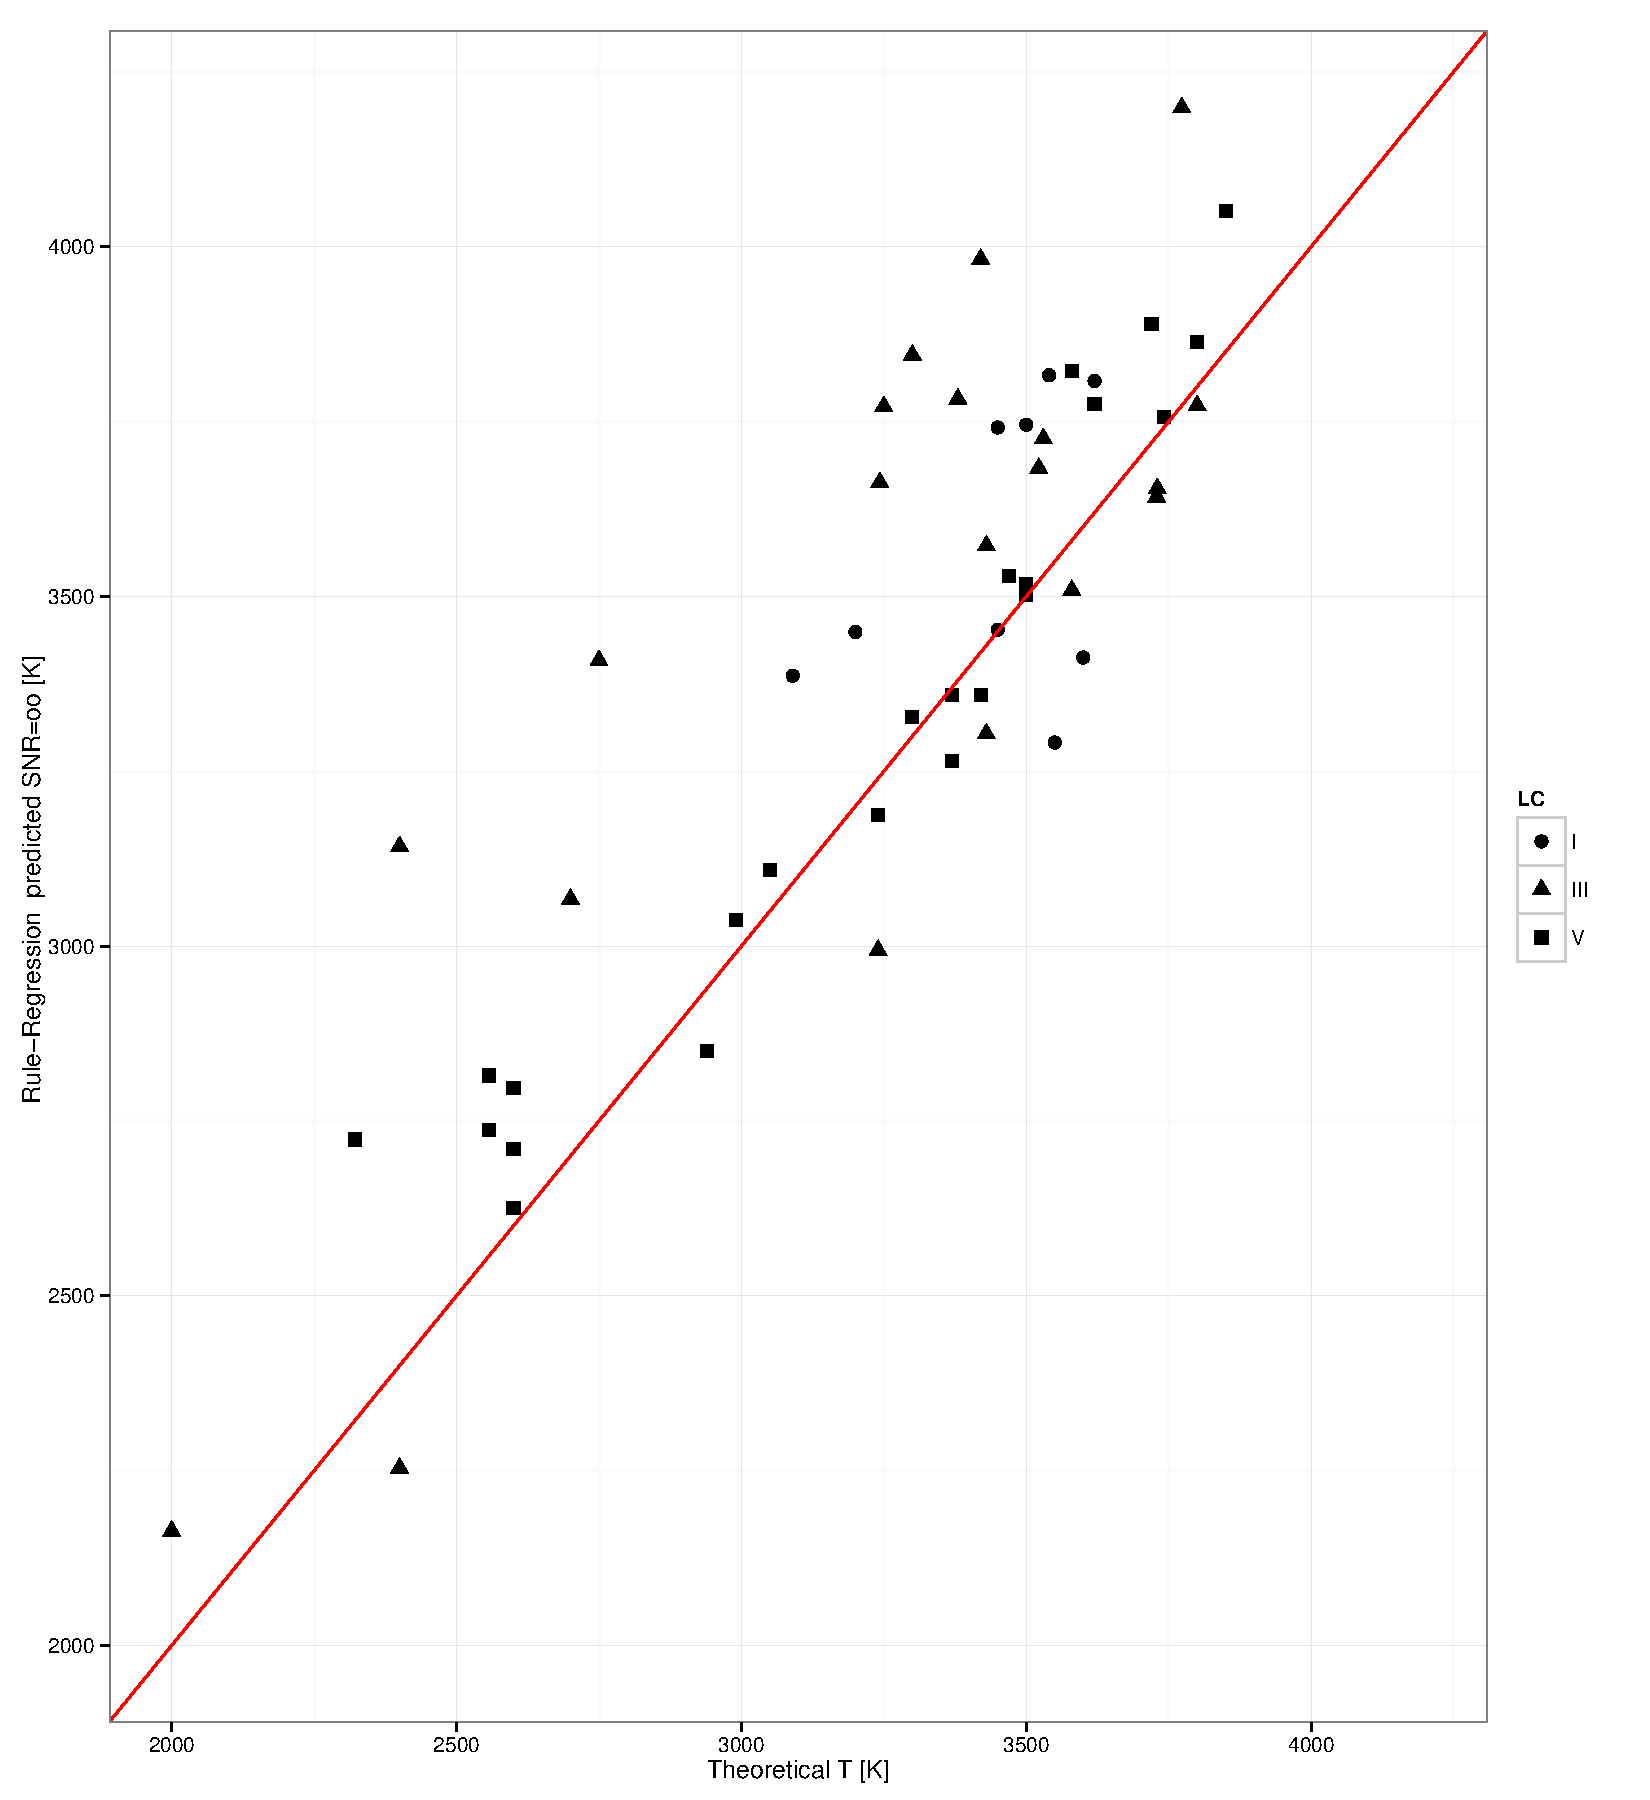
\includegraphics[width=11cm]{figs/irtf_T_rreg50_Cesetti.pdf}
  \caption{Comparison between Temperature estimations from Cesetti 
 in x axis and the Rule Regression model for GA based features 
 at SNR=$50$ on y-axis}
 \label{fig:ga_rr50ga_spt}
 \end{subfigure} 
 \label {fig:comp02}
 \caption{Performance comparison between two Rule regression based models with different SNR}
\end {figure}

%%%%%%%%%%%%%%%%%%%%%%%%%%%%%%%%%%%%%%%%%%%%%%%%%%%%%%%%%%%%%%
% Comparison with Teffs from spectral types.
%%%%%%%%%%%%%%%%%%%%%%%%%%%%%%%%%%%%%%%%%%%%%%%%%%%%%%%%%%%%%%

We then compare the predicted effective temperatures with the spectral
types listed in the IRTF spectral library in order to increase the
size of the validation sample beyond the 57 cases with estimated
temperatures in Table 3 of \cite{cesetti}. We converted the spectral
types into effective temperatures using the calibration of
\cite{2009ApJ...702..154S}. Both the RMSE and RMDSE were used to
evaluate the prediction accuracy (see Table~\ref{tab:model_Tvar}).

{\bf Faltan las tablas y figuras.}



%%%%%%%%%%%%%%%%%%%%%%%%%%%%%%%%%%%%%%%%%%%%%%%%%%%%%%%%%%%%%%
% TBD: Comparison with temperatures estimated with Cesetti features
%%%%%%%%%%%%%%%%%%%%%%%%%%%%%%%%%%%%%%%%%%%%%%%%%%%%%%%%%%%%%%

We have trained the same non linear regression models discussed above
using the features suggested by \cite{cesetti}. The performace of the
models based on these features are included in Table
\ref{tab:tab_CS_Model}.

\begin{table}\centering
\ra{1.3}
\begin{tabular}{@{}rrrcrrcrr@{}}\toprule
& \multicolumn{2}{c}{$SNR = 10$} & \phantom{ab}& \multicolumn{2}{c}{$SNR = 50$} &
\phantom{ab} & \multicolumn{2}{c}{$SNR = \infty$}\\
\cmidrule{2-3} \cmidrule{5-6} \cmidrule{8-9}
$Regression Models$ & $RMSE$ & $RMDSE$ && $RMSE$ & $RMDSE$ && $RMSE$ & $RMDSE$ \\ \midrule
CS-RF               & 234       & 180       && {\bf 264} & 218       &&  {\bf 321} & 265 \\
CS-GBM              & {\bf 232} & 195       && 268       & 254       &&  325       & 246 \\
CS-SVR              & 268       & 227       && 293       & 257       &&  432       & 364 \\
CS-NNET             & 357       & 255       && 357       & {\bf 204} &&  552       & 435 \\
CS-KNN              & 249       & 172       && 293       & 256       &&  327       & {\bf 230}\\
CS-KPLS             & 351       & {\bf 162} && 856       & 456       && 1086       & 535 \\
\hline
\end{tabular}
\caption {Regression model performance based on the features proposed by \cite{cesetti}} 
\label{tab:tab_CS_Model}
%\end{center}
\end{table}

{\bf How do you explain that the best SNR=10 model has the poorest
  performances for SNR=50 or $\infty$?}

From the comparison of Tables \ref{tab:tab_CS_Model} and
\ref{tab:model_TSD} we can draw the following conclusions:

\begin{itemize}
\item the RMSE for SNR=10 and 50 is equivalent for the regression
  models trained on GA features and those recommended in
  \cite{cesetti};
  \item however, the RMDSE is significantly higher in the case of the
    latter features for all SNR values.
    \item in the unrealistic case of noiseless spectra, the features
      proposed by \cite{cesetti} produce RMSE and RMDSE significantly
      worse than the GA features.
\end{itemize}

As a summary, we believe that the features found by the GA are to be
prefered to the ones proposed by \cite{cesetti}.

\subsection{Surface gravity models}

For the validation of our models, we only have 10 literature values of
the surface gravity available in Table 3 of
\cite{cesetti}. Unfortunately, this is too small a number to draw
significant conclusions on the comparison of methodologies from
external data. Hence, we are left only with plausibility arguments for
the selection of models. In this Section we will use $\log(T_{\rm
  eff})--\log(g)$ diagram comparisons to select the most plausible
model results. An important difference with respect to the models
discussed above is that we use the $T_{\rm eff}$ estimated in the
previous stage as input of our models. {\bf do we have some hint
  whether this was beneficial, neutral or detrimental?}

Table~\ref{tab:models_G_rmse} shows the RMSE and RMDSE of the
$\log(g)$ regression models for the same SNR regimes discussed for the
estimation of $T_{\rm eff}$.

\ra{1.3}
\begin{table*}\centering
\begin{tabular}{@{}rrrcrrcrr@{}}\toprule
& \multicolumn{2}{c}{$SNR = 10$} & \phantom{ab}& \multicolumn{2}{c}{$SNR = 50$} &
\phantom{ab} & \multicolumn{2}{c}{$SNR = \infty$}\\
\cmidrule{2-3} \cmidrule{5-6} \cmidrule{8-9}
$Regression Models$ & $RMSE$ & $RMDSE$ && $RMSE$ & $RMDSE$     && $RMSE$       & $RMDSE$ \\ \midrule
$\chi^2$          & 0.82       & 0.45      && 0.93       & 0.61       && 3.5        & 3.48 \\
$ PPR-ICA$        & 0.54       & 0.48      && {\bf 0.3}  & {\bf 0.17} && 0.72       & 0.57 \\
GA-RF             & 0.64       & \bf{0.38} && 0.77       & 0.72       && 0.53       & 0.39 \\
GA-GBM            & {\bf 0.48} & 0.45      && 0.61       & 0.47       && 0.49       & 0.41 \\
GA-SVR            & 0.66       & 0.40      && 0.63       & 0.58       && {\bf 0.46} & \bf{0.21} \\
GA-NNET           & 0.78       & 0.61      && 0.47       & 0.44       && 1.2        & 0.97 \\
GA-MARS           & 0.84       & 0.57      && 0.54       & 0.37       && 0.99       & 0.76 \\
GA-KNN            & 1.23       & 0.83      && 1.39       & 1.44       && 1.60       & 1.32 \\
GA-KPLS           & 0.99       & 0.99      && 0.51       & 0.49       && 0.96       & 0.77 \\
GA-RR             & 0.74       & 0.57      && 0.50       & 0.47       && 0.57       & 0.41 \\

\bottomrule
\end{tabular}
\caption {RMSE and RMDSE for the various $\log(g)$ regression models
  [dex].}
\label{tab:models_G_rmse} 
% \end{center}
\end{table*}

Again, as in the case of the effective temperatures, the differences
between the various models as measured by the RMSE or RMDSE are not
statistically significant.  This is not surprising given the
extraordinarily small sample of gravity measurements gathered from the
literature and used as reference for the computation of errors.
However, we can evaluate the models according to plausibility
arguments relative to the distribution of the model predictions in
$T_{\rm eff}$--$\log(g)$ diagrams.  Figure~\ref{fig:lt_lg_ga} shows
this distribution for four models selected based on these plausibility
criteria: GA-RR, GA-PLS, GA-KNN (the three of them for SNR=50), and
PPR-ICA (clockwise, starting at the top left corner).

\begin{figure}
 \begin{center}
   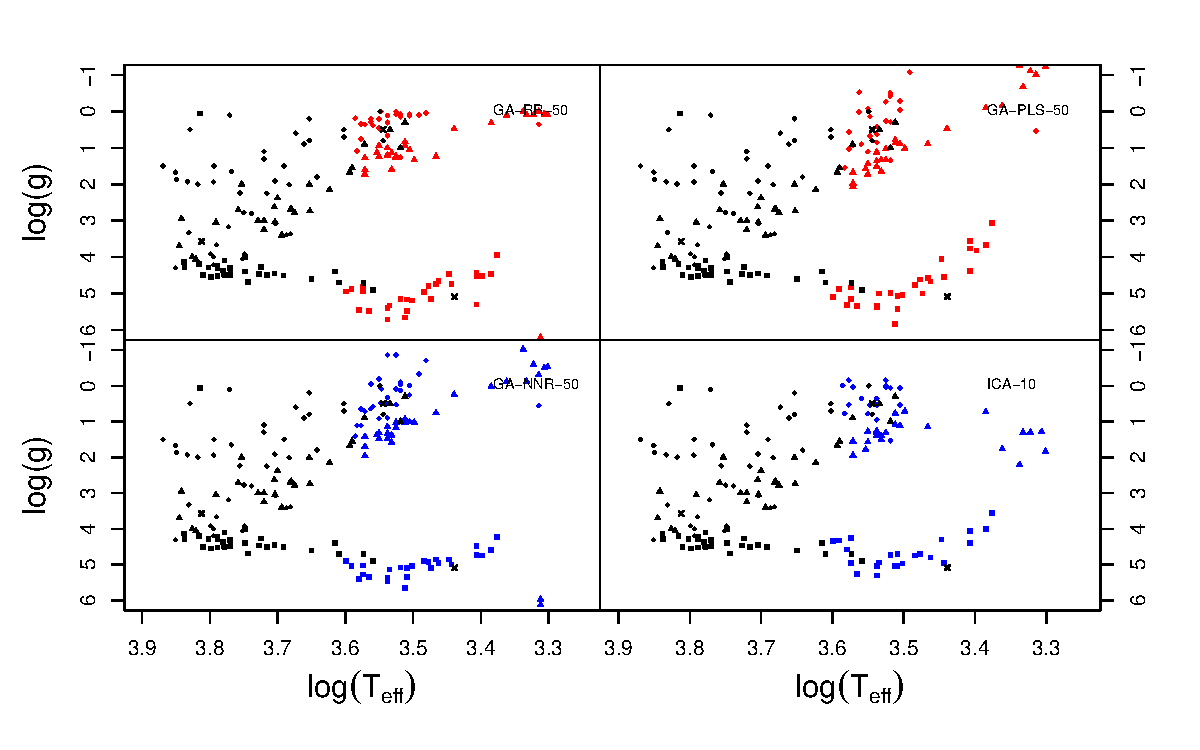
\includegraphics[width=\textwidth]{figs/ordieres-fig4.pdf}
 \caption{$\log(T_{eff})$--$\log(g)$ diagrams produced by the GA-KNN
   (SNR=$\infty$) effective temperatures and gravities derived with
   the GA-RR (SNR=50), GA-PLS (SNR=50), GA-NNR (SNR=50), and $\chi^2$ models (clockwise, starting from
   the top left plot).}
 \label{fig:lt_lg_ga}
 \end{center}
\end{figure}

{\bf Is $\chi^2$ much worse now for the weak parameter logg? I guess
  no. This needs be discussed}

{\bf Discuss these plots in the case of Cesetti features.}

\subsection{Metallicity models} 

Finally, the same machine learning models are trained to infer the
metallicity, again considering the effective temperature as an input
feature as in the $\log(g)$ regression
models. Table~\ref{tab:models_M_rmse} shows the RMSE and RMDSE
obtained for each regression model for the only seven M-type stars in
Table 3 of \cite{cesetti} with a metallicity estimate in the
literature.
%
% Metalicidad teórica desde Cesseti para las IRTF
%
\ra{1.3}
\begin{table*}\centering
\begin{tabular}{@{}rrrcrrcrr@{}}\toprule
& \multicolumn{2}{c}{$SNR = 10$} & \phantom{ab}& \multicolumn{2}{c}{$SNR = 50$} &
\phantom{ab} & \multicolumn{2}{c}{$SNR = \infty$}\\
\cmidrule{2-3} \cmidrule{5-6} \cmidrule{8-9}
$Regression Models$ & $RMSE$ & $RMDSE$ && $RMSE$ & $RMDSE$     && $RMSE$       & $RMDSE$ \\ \midrule
$\chi^2$    & 0.76 & 0.22      && 0.36 & 0.18     && 0.36 & 0.18 \\
$PPR-ICA$   & 0.24 & \bf{0.13} && 0.31 & 0.22     && 0.43 & 0.27 \\
$GA-RF$     & 0.33 & 0.25      && 0.73 & 0.41     && 0.61 & 0.36 \\
$GA-GBM$    & 0.27 & 0.19      && 0.70 & 0.52     && 0.63 & 0.35 \\
$GA-SVR$    & 0.33 & 0.22      && 0.45 & 0.32     && 0.92 & 0.89 \\
$GA-NNET$   & 0.37 & 0.30      && 0.33 & 0.37     && 0.95 & 0.81 \\
$GA-KNN$    & 0.69 & 0.55      && 0.23 & \bf{0.15}&& 0.21 & \bf{0.15} \\ 
$GA-MARS$   & 0.36 & 0.16      && 0.49 & 0.41     && 0.83 & 0.85 \\
$GA-RR$     & 0.31 & 0.17      && 0.30 & 0.24     && 0.78 & 0.23 \\

\bottomrule
\end{tabular}
\caption {RMSE and RMDSE for the various regression models predicting
  metallicity [dex].}
\label{tab:models_M_rmse} 
% \end{center}
\end{table*}



{\bf Compare the 7 or 6 values available. Discuss.  $\chi^2$ is
  the most popular method by far. We compare predictions of machine
  learning methods with minimum chi-squared. We first do histogram
  plots. Then, the same logTeff-logg plots as above but with
  metallicity coded in colour.}

% To be corrected
 Figure~\ref{M_ICA_10} shows the relationships between metalicity
 predicted by global espectrum estimation and GA feature based
 estimation against the real values provided by
 \cite{2013A&A...549A.129C} can be observed.

 \begin {figure}
  \centering
   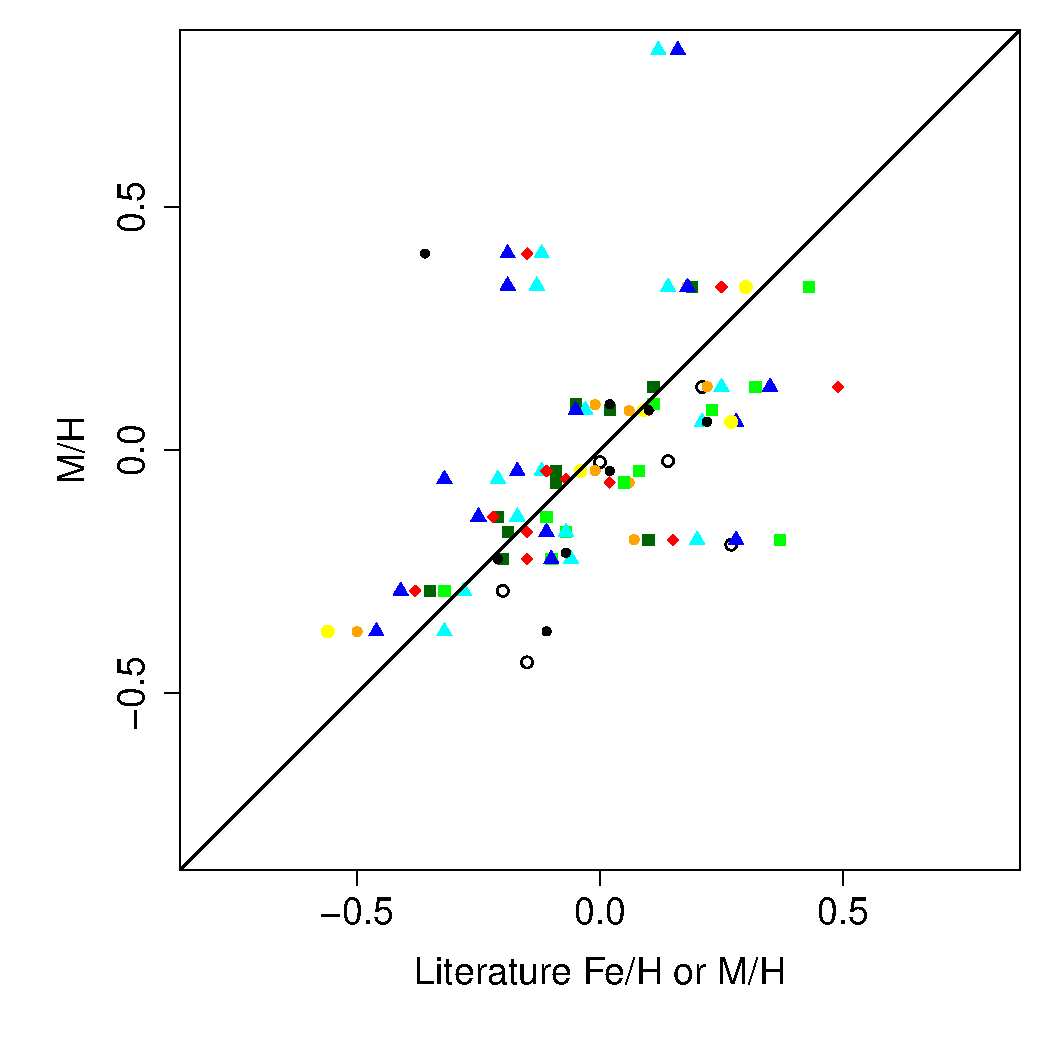
\includegraphics[width=\textwidth]{figs/teff-logg/M-ICA10.pdf}
   \caption{Comparison between metallicity estimates from the
     literature and predictions from the PPR-ICA (SNR=10) model. {\bf
       TBC: Include description of symbols and colours.}}
  \label{M_ICA_10}
 \end {figure}

 {\bf Include table as annex with metallicities from the literature.}
